\begin{abstract}
Pretraining can make the encoder itself less readable while its objective improves. We identify a mechanism: redistribution of readable directions at preserved rank. For convolution, squaring, and global pooling, local second moments give an exact feature dictionary. Correlated filters and head coupling move the encoder's prediction space even under an isotropic objective. In an explicit joint parameter gradient flow with a genuine encoder bottleneck, a prespecified task cone uniformly improves and then exceeds its initial risk, for both encoder and projection. The encoder increase rules out head selection as the sole cause; optimal unregularized population probes remove finite-label fitting and invertible feature scaling as explanations. A quantitative stability theorem preserves positive gaps under independent perturbations of all six initialization coordinates in a small explicit neighborhood, establishing rebound beyond the exact symmetric trajectory. Finite-data texture training additionally yields complete encoder rebound for seven fixed tasks in one or two of six new seeds, at comparison times fixed using earlier runs; matched linear and frozen-encoder controls yield none. Short-horizon predictions and natural-image diagnostics delimit the scope. Together, these results identify how continued objective descent can rotate a fixed-dimensional encoder space away from task-relevant directions.
\end{abstract}

\section{Introduction}
\label{main:introduction}
Pretraining optimizes one objective, while a later task reads the resulting representation. A decreasing objective can coexist with worse task performance, but that observation alone does not identify a mechanism. Output rescaling, a regularized probe, compression by a head, and movement of the encoder's prediction space can produce different apparent effects. We isolate the last mechanism using optimal, unregularized population linear risk. Its invariance to invertible feature rescaling makes a risk increase evidence about task readability rather than feature magnitude.

Our model is convolution followed by squaring, global average pooling, and a linear projection. Its centered outputs are linear functions of a local second-moment dictionary for every input distribution. Standard population regression then evaluates a task against a representation subspace. The dynamical question is which actual parameter updates leave that subspace and how the moving space intersects task directions.

The core result concerns a genuine encoder bottleneck: one projected output, two encoder channels, and three independent quadratic statistics. Correlated filters create exterior encoder motion even when the objective is isotropic. An explicit solution shows a quadratic direction approaching a task cone and then moving past it. The same two geometric sections improve and subsequently exceed the initial risks for the entire cone. Both encoder and projection have fixed positive gaps while their ranks stay constant and pretraining loss decreases.

The solvable trajectory has a reflection symmetry, but rebound persists when all four filter coordinates and both head entries vary independently in an explicit box. At fixed data, rates, and nonzero augmentation, angular and imbalance equations control the task projectors through a directional progress clock. We prove first arrival, bounded parameters, preserved ranks, and finite physical time. This turns an exactly solvable trajectory into a parameter region with the same task-uniform improvement and rebound.

Controlled textures test complete rebound beyond the analytic family using independent nonsymmetric initializations. Ten tasks are fixed; earlier seeds select two comparison times and a risk-amplitude threshold before six new seeds are run. Seven tasks each rebound in one or two new seeds, while three never do; matched linear and frozen-encoder controls yield no encoder rebounds. Exact population risks at finite-data SGD checkpoints remove fitted-probe error. These observations establish instances beyond the construction, with limited task-wise frequency and no random-initialization typicality claim.

Four features make the result informative. Encoder risk rises, so changing the head alone cannot recover the lost linear readability. Rank stays fixed, so the mechanism reallocates readable directions without dimensional collapse. The probe is population-optimal and unregularized, so finite-label estimation and invertible feature scaling cannot produce the rebound. Finally, independent initialization perturbations preserve the gaps, so exact symmetry is sufficient for solving the flow but unnecessary for the phenomenon. Task-coupling bounds interpret this mechanism; rate comparisons, a projection certificate, conditional stochastic propositions, and detailed diagnostics appear in the supplement.

\section{Related Work}
\label{main:related}
\paragraph{Optimization geometry.}
Kunin et al.~\cite{kunin2024rich} solve supervised two-layer linear dynamics and show how layer imbalance and learning rates change feature learning, including matched initial functions. Their rotating trajectories provide a precedent for nonmonotonic readability of a separately chosen task. Here an unsupervised moment objective and square parameterization yield task-uniform finite risk gaps in the encoder itself, with quantitative initialization stability.

\paragraph{Projection and task selection.}
Gui et al.~\cite{gui2023projection} characterize expansion and shrinkage with a fixed encoder. Xue et al.~\cite{xue2024benefits} analyze feature weighting and information differences across nonlinear heads. Torralba and Weiss~\cite{torralba2026theory} study the same broad convolution--nonlinearity--pooling architecture and GUPA objective, including initialization and recognition degradation. Our encoder/projection separation identifies a loss that head selection alone cannot explain: even the encoder's best population linear decoder worsens during joint training.

\paragraph{Nonlinearity and collapse.}
Jing et al.~\cite{jing2022collapse} study dimensional collapse in linear contrastive training; Tian~\cite{tian2023nonlinearity} analyzes nonlinear contrastive dynamics. Here the encoder reorients at preserved rank: its capacity to read different quadratic directions changes while its dimension stays fixed. This distinguishes task-specific readability loss from dimensional collapse. Supplement Sec.~\ref{supp:literature} compares assumptions, training dynamics, and risk objects.

\paragraph{Geometric overshoot and quadratic dynamics.}
Yang, Saxe, and Latham~\cite{yang2026abstraction} prove finite-time overshoot and residence-time results for abstraction alignment with an instantaneously ridge-optimal readout. We evaluate the best unregularized population decoder while the pretraining head follows joint finite-rate dynamics, separating task-space movement from readout regularization. Neural quadratic forms~\cite{liu2026nqf} provide moment closure and exact Riccati dynamics, while Yang~\cite{yang2026spectral} analyzes teacher-dependent quadratic loss histories and identifiability. These establish close dynamical tools. The trainable head matters to our parameter metric: absorbing a positive head into a quadratic filter preserves its function but generally changes Euclidean training.

\section{Task Geometry and Exterior Encoder Motion}
\label{main:geometry}
\subsection{Moment dictionary and task risk}
For valid image patches $p_u(x)\in\R^p$, define
\begin{align}
 M(x)&=|U|^{-1}\sum_u p_u(x)p_u(x)^\top,\nonumber\\
 r_c(x)&=h_c^\top M(x)h_c.
\end{align}
Let $\phi=\operatorname{svec}(M-\E M)$, using isometric symmetric vectorization. Write its covariance on its support as $U\Lambda U^\top$, $\Lambda\succ0$. Then
\begin{align}
 u&=\Lambda^{-1/2}U^\top\phi,\qquad \E uu^\top=I,\\
 B_{c:}&=\operatorname{svec}(h_ch_c^\top)^\top U\Lambda^{1/2},\qquad A=WB.
 \label{main:moment-map}
\end{align}
The centered encoder and projection are exactly $Bu$ and $Au$, without Gaussian or independent-frequency assumptions. Augmentation-only covariance directions must also be retained when computing training gradients.

For centered labels $Y$ with finite second moment, set $C_Y=\E[uY^\top]$ and $T=C_YC_Y^\top$. Standard affine least squares gives
\begin{equation}
 R(A)=\tr\operatorname{Cov}(Y)-\tr(P_AT),\qquad P_A=A^\dagger A.
 \label{main:task-risk}
\end{equation}
For $Y=\beta^\top u$ and $\norm\beta=1$, this is $1-\beta^\top P_A\beta$; encoder risk substitutes $B$. Labels need not be linear in $u$ for the general identity. This is linear readability, not all task information or finite-sample probe generalization.

This distinction separates two mechanisms. Since $A=WB$, $\row A\subseteq\row B$: a head may fail to select a readable encoder direction. In contrast, a change in $P_B$ changes which linear functions of the fixed moment dictionary the encoder can predict. Neither effect requires a change in rank. Indeed, for a complete orthonormal set of unit coordinate tasks,
\begin{equation}
 \sum_{j=1}^{d}R_{e_j}(B)=d-\operatorname{rank}(B).
\end{equation}
At fixed rank, training redistributes a readability budget among directions. The central question is whether actual filter updates rotate that budget away from an independently specified task, rather than merely alter the weights of accessible features.

\subsection{Objective and actual parameter metric}
For view covariance $\Sigma=ASA^\top$ and view-difference moment $D$, use GUPA~\cite{torralba2026theory} directly:
\begin{align}
 L(A)={}&\tfrac12\tr(ADA^\top)-\tfrac12\log\det(I+\Sigma)\nonumber\\
 &-\tfrac12\tr\big((I+\Sigma)^{-1}\Sigma\big).
 \label{main:gupa}
\end{align}
The quadratic embeddings are not Gaussian, and no exact InfoNCE equivalence is assumed. For isotropic view moments $S=sI$, $D=2(s-1)I$ and one output, $L=\Phi(V)$, $V=\norm A^2$. Independent Gaussian view noise of relative power $\eta$ gives $s=(1+\eta)^2$ and
\begin{equation}
 \Phi(V)=(s-1)V-\tfrac12\log(1+sV)-\frac{sV}{2(1+sV)}.
\end{equation}
Here $V$ is clean-output energy and $Q=sV$ is single-view variance; the energy condition $Q<1$ uses this same quantity throughout. We train Euclidean filters and head rather than optimizing $A$ freely. For $G=\nabla_AL$ and $J_h=D_h(WB)$,
\begin{equation}
 \dot A=-\eta_hJ_hJ_h^*[G]-\eta_WGB^\top B.
 \label{main:parameter-mobility}
\end{equation}
Its exterior component determines whether the representation space changes.

\subsection{A concrete motion criterion}
At fixed full row rank, $P=P_A$ satisfies
\begin{equation}
 \dot P=A^\dagger\dot A(I-P)+(I-P)\dot A^\top(A^\dagger)^\top.
\end{equation}
Large gradient or growing energy alone does not ensure task change. For a linear factorization $A=WV$ and $G=HA+E$,
\begin{equation}
 \dot V(I-P_V)=-\eta_VW^\top E(I-P_V).
 \label{main:linear-normal}
\end{equation}
The isotropic part $HA$ preserves the encoder space; residual anisotropy can move it. Exact isotropic conservation also holds for ordinary discrete gradient descent when $V$ retains rank, since each update left multiplies $V$.

For GUPA this residual is explicit. Write $S=sI+\Delta S$, $D=d_0I+\Delta D$, and
\begin{equation}
 K_A=(I+ASA^\top)^{-1}+(I+ASA^\top)^{-2}.
\end{equation}
Then $G=AD-K_AAS$ gives $H=d_0I-sK_A$ and $E=A\Delta D-K_AA\Delta S$, with
\begin{equation}
 \norm E_F\le\norm A_F(\norm{\Delta D}_2+2\norm{\Delta S}_2).
\end{equation}
Together with Equation~\eqref{main:linear-normal}, this identifies an objective-moment source of linear drift. A near-isotropic training distribution need not give exact conservation, even if the architecture is linear.

For square filters, write $H_c=h_ch_c^\top$ and $\mathcal S=\operatorname{span}\{H_c\}$. With isotropic Gaussian patches, $B_{c:}=\sqrt2\operatorname{svec}(H_c)^\top$. If $G=HA$ with symmetric $H$, put $K_0=W^\top HW$. Exterior updates are determined by
\begin{equation}
 \Pi_{\mathcal S^\perp}\sum_j(K_0)_{cj}(H_cH_j+H_jH_c).
\end{equation}
Thus parameter mobility can move the encoder even with isotropic objective moments. For two linearly independent filters, let $\rho_h=h_1^\top h_2$, $Q_B=I-P_B$, and
$n=Q_B\operatorname{svec}(h_1h_2^\top+h_2h_1^\top)$. Then
\begin{equation}
 \dot BQ_B=-4\sqrt2\eta_h(K_0)_{12}\rho_h(1,1)^\top n^\top.
 \label{main:two-filter-normal}
\end{equation}
Because $n\ne0$, the encoder moves exactly when correlation and objective/head coupling are both nonzero. Orthogonal filters exclude motion. This equivalence is specific to two independent channels: additional channels may span a cross quadratic or cancel its contribution. The supplement gives the mobility derivation and near-isotropy bounds.

The algebra shows why squaring changes the conclusion. A filter update creates the cross statistic $h_ch_j^\top+h_jh_c^\top$, multiplied by $h_c^\top h_j$. With two independent filters, that statistic is outside the span of their two squares; with orthogonal filters its coefficient vanishes. This is a condition on the current filters and head, rather than on nonlinearity alone.

The same calculation distinguishes motion from its task effect. Put $p=B^\dagger(1,1)^\top$ and $v=-4\sqrt2\eta_h(K_0)_{12}\rho_hp$. Equation~\eqref{main:two-filter-normal} yields
\begin{equation}
 \dot P_B=vn^\top+nv^\top,\qquad v\perp n.
\end{equation}
When $v\ne0$, the unit tasks $\beta_\pm=(v/\norm v\pm n/\norm n)/\sqrt2$ have opposing risk derivatives of magnitude $\norm v\norm n$. A task along $n$ instead has zero first derivative. Thus even a single nonzero exterior update can improve one task, hurt another, and be first-order invisible to a third. This local observation motivates the finite-amplitude task-family theorem below; it does not itself establish a persistent risk change.

\section{Encoder Rebound and Quantitative Stability}
\label{main:rebound}
\subsection{A solvable encoder rebound family}
\label{sec:bottleneck-family}
The following family makes the mechanism explicit in a genuine bottleneck $K=1<C=2<d=3$. Its moving directions are coupled quadratic statistics, not an embedding with dormant extra coordinates.

Let $x\sim N(0,\Sigma_x)$ be one two-dimensional patch, with
\begin{equation}
 \Sigma_x=\nu_+e_+e_+^\top+\nu_-e_-e_-^\top,
 \qquad \nu_\pm\in[19/20,21/20],
\end{equation}
where $e_+,e_-$ are orthonormal. Write $q_c=\Sigma_x^{1/2}h_c$ for the filters in whitened input coordinates, and initialize
\begin{align}
 q_1&=\sqrt\epsilon\,e_++\sqrt{\epsilon/2}\,e_-,\\
 q_2&=\sqrt\epsilon\,e_+-\sqrt{\epsilon/2}\,e_-,\qquad W=(w_0,w_0).
\end{align}
Set $E_\pm=e_\pm e_\pm^\top$ and $E_\times=(e_+e_-^\top+e_-e_+^\top)/\sqrt2$. These give orthonormal coordinates for
\begin{equation}
 u=\operatorname{svec}(yy^\top-I)/\sqrt2,\qquad y=\Sigma_x^{-1/2}x.
\end{equation}
For tasks use the unit vector associated with the symmetric matrix
\begin{equation}
 \beta_{\psi,z}=\sqrt{1-z^2}(\cos\psi E_++\sin\psi E_-)+zE_\times.
\end{equation}

\begin{theorem}[Uniform encoder and projection risk gaps]
\label{thm:bottleneck-family}
Let $0<\epsilon\le1/100$, $0<w_0\le1/10$, $\eta_h>0$, and $0\le r=\eta_W/\eta_h\le10$. Use GUPA with views $x+\xi_j$, where independent $\xi_j\sim N(0,\eta\Sigma_x)$ and $0\le\eta\le1/5$. Train the actual Euclidean parameters $h,W$. Put $\theta_0=\arctan(1/2)$. For every task $Y=\beta_{\psi,z}^\top u$ with
\begin{equation}
 2\theta_0/3\le\psi\le5\theta_0/6,\qquad |z|\le1/2,
\end{equation}
the same two comparison states $t_1<t_2$ satisfy, for both optimal encoder and projection risks,
\begin{align}
 R(t_1)&\le R(0)-\Delta_1,\\
 R(t_2)&\ge R(0)+\Delta_2,
\end{align}
where
\begin{align}
 \Delta_1&=\tfrac34\sin(\theta_0/4)\sin(\theta_0/12)>0.00335,\\
 \Delta_2&=\tfrac34\sin(5\theta_0/6)\sin(\theta_0/6)>0.02181.
\end{align}
Both states are reached before $t_2<5/(76\eta_hw_0^2\epsilon)$; the loss strictly decreases and the encoder/projection ranks remain two/one. Changing $r$ in this family changes speed and energy, but not the ordered subspace path or these gaps.
\end{theorem}

\paragraph{Mechanism and exact solution.}
Equal head entries and the displayed filter symmetry persist. Put $\lambda_\pm=\norm{q_1}^2\pm q_1^\top q_2$ and $\kappa=2\Phi'(V)$ for the radial objective $L=\Phi(V)$, $V=\norm A^2$. In the increasing clock $\tau=-8\eta_h\int\kappa w^2dt$,
\begin{align}
 \lambda_\pm(\tau)&=\frac{\lambda_\pm(0)}{1-\nu_\pm\lambda_\pm(0)\tau},\\
 w^2&=w_0^2+\frac r4\sum_{j\in\{+,-\}}
             \frac{\lambda_j-\lambda_j(0)}{\nu_j}.
 \label{eq:analytic-family}
\end{align}
The encoder retains $E_\times$ and the diagonal direction $\lambda_+E_++\lambda_-E_-$; the projection retains only the latter. Its angle $\theta=\arctan(\lambda_-/\lambda_+)$ strictly decreases. The task risks are exactly
\begin{align}
 R_{\rm enc}&=(1-z^2)\sin^2(\theta-\psi),\\
 R_{\rm proj}&=z^2+(1-z^2)\sin^2(\theta-\psi).
 \label{eq:analytic-risks}
\end{align}
The two common states are $\theta_1=3\theta_0/4$ and $\theta_2=\theta_0/6$. Motion first approaches the task direction and then continues past it; the encoder itself loses readability. The fixed projection gap $z^2$ is a separate selection effect.

\begin{figure}[t]
\centering
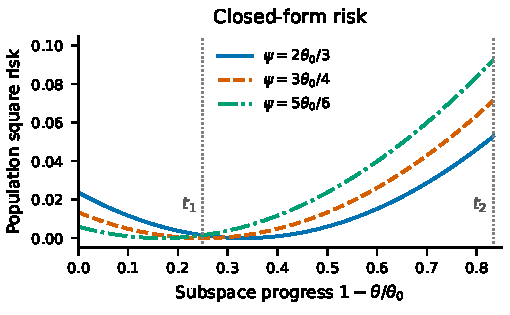
\includegraphics[width=\linewidth]{figures/analytic_bottleneck_family.pdf}
\caption{Exact risk paths in Theorem~\ref{thm:bottleneck-family}, three task directions with $z=0$. Encoder and projection risks coincide here. The same two comparison states improve and then exceed the initial risk for the entire task family. These curves evaluate the closed formula; no model is trained or numerically integrated to draw them.}
\label{fig:analytic-family}
\end{figure}

The task family contains an open cone and covers a specified $\pm5\%$ covariance range. This anisotropy range keeps covariance axes aligned with filter sums/differences and uses covariance-relative augmentation and balanced whitened initialization. Physical initial filters change with the covariance to keep that whitened balance. It is not robustness to arbitrary symmetry-breaking initialization or augmentation perturbations, nor a random-initialization probability result. The family also supplies an explicit exclusion case for rate competition: unequal rates alone do not force different directional paths. Appendix~\ref{app:task-geometry} proves the formulas, energy barrier, and reachability.


\section{Which Motion Changes a Task?}
\label{main:task-coupling}
For equal-rank projectors $P_0,P_1$, put $Q_0=I-P_0$, $a_0=\norm{Q_0TP_0}_F$, and $d=\norm{P_1-P_0}_F/\sqrt2$. Exact row/normal block decomposition gives
\begin{equation}
 |R(P_1)-R(P_0)|\le2a_0d+\operatorname{osc}(T)d^2.
 \label{main:finite-task-bound}
\end{equation}
Small displacement and weak task cross coupling separately limit risk amplitude. A zero cross block removes the first-order term, not all finite effects.

To see what the bound retains, define
\begin{align}
 U_1&=P_0(I-P_1)P_0,\quad V_1=Q_0P_1Q_0,\nonumber\\
 Z_1&=Q_0P_1P_0.
\end{align}
The exact risk difference is
\begin{align}
 \Delta R={}&\tr(P_0TP_0U_1)-\tr(Q_0TQ_0V_1)\nonumber\\
 &-2\tr(P_0TQ_0Z_1).
 \label{main:finite-block-identity}
\end{align}
Both $U_1,V_1$ are PSD with trace $d^2$, while $\norm{Z_1}_F\le d$. The cross term couples the direction of motion to the task; the two diagonal terms account for finite leakage out of and into the initial space. Bounding them gives Equation~\eqref{main:finite-task-bound}. A displacement-only bound discards the cross term's orientation, and therefore assigns the same budget to tasks with very different responses.

There are also exclusion cases. If $T$ is a scalar multiple of the identity, risk is constant at fixed rank. If $P_0TQ_0=0$ and the smallest eigenvalue of the task's row block exceeds the largest eigenvalue of its normal block by $\delta>0$, Equation~\eqref{main:finite-block-identity} gives $\Delta R\ge\delta d^2$. Every departure then worsens this task; initial improvement is impossible. These checks clarify why encoder motion alone cannot predict a rebound curve.

This task dependence separates encoder movement from its risk effect: each fixed task must be tested against the moving space. It also motivates pairing source motion with tasks in the supplementary prediction analysis. Supplement Sec.~\ref{supp:stochastic-framework} develops conditional stochastic propositions separating source calibration, predictable drift, step curvature, and centered task variance. Their support/tail and variance-confidence assumptions are distinct from the empirical calibration used in our experiments.

\section{Controlled Texture Evidence and Boundaries}
\label{main:experiments}
\paragraph{Fixed tasks and independent training.}
Periodic $32\times32$ textures contain 16 independent non-DC power coordinates: four directions, two radial bands, and two frequency pairs per group. Ten fixed unit-variance tasks comprise two coordinates and eight direction/band sums. We train eight square channels and one head output using true full-support pixel kernels, evaluating their periodic-image forward exactly in the Fourier dictionary. Training uses 32,768 unlabeled samples, batch size 256, 4,000 SGD updates, learning rate $0.002$, augmentation power $0.2$, and unit head/front rate ratio. Task risks are exact optimal unregularized population risks for the known synthetic distribution; labels enter evaluation only.

\paragraph{Complete encoder rebound beyond the construction.}
We use earlier seeds 2--11 to develop comparison times 1,000/4,000 and threshold $\delta=10^{-3}$, then fix them before running new seeds 20--25. For each prespecified task, a complete rebound requires both
\begin{equation}
 I=R(0)-R(1000)>\delta,\quad D=R(4000)-R(0)>\delta.
 \label{main:empirical-rebound-rule}
\end{equation}
Independent Gaussian filter/head draws undergo stated, label-free energy and mobility-trace calibration; they do not satisfy the two-filter symmetry. All 18 model/seed trajectories complete. Seven fixed tasks each rebound in one or two seeds; the other three yield none (Table~\ref{main:rebound-counts}). Tasks within a seed are correlated, and six seeds do not estimate occurrence probabilities precisely. Descriptively, five seeds have at least one successful task; none has all ten.

\begin{figure}[t]
\centering
\includegraphics[width=\linewidth]{figures/encoder_rebound_x_low.pdf}
\caption{Fixed-task encoder risk relative to its own initialization, all six seeds and three models. The task $x_{\rm low}$ is an illustrative display; Table~\ref{main:rebound-counts} retains every fixed task. Lines mark updates 1,000/4,000 and thresholds $\pm10^{-3}$. A complete rebound crosses below the negative threshold at the first comparison and above the positive threshold at the second.}
\label{main:encoder-rebound}
\end{figure}

\begin{table}[t]
\centering\small
\caption{Complete encoder rebound at the fixed times and threshold in Equation~\eqref{main:empirical-rebound-rule}. Every entry retains all six planned seeds. These are task-wise counts, not independent task repetitions.}
\label{main:rebound-counts}
\setlength{\tabcolsep}{4pt}
\begin{tabular}{lrrr}
\toprule
Fixed task&Square&Linear&Frozen\\\midrule
single $x$ low&2/6&0/6&0/6\\
single $y$ low&1/6&0/6&0/6\\
$x$ low&2/6&0/6&0/6\\
$x$ high&0/6&0/6&0/6\\
$y$ low&2/6&0/6&0/6\\
$y$ high&0/6&0/6&0/6\\
diagonal low&1/6&0/6&0/6\\
diagonal high&0/6&0/6&0/6\\
antidiagonal low&1/6&0/6&0/6\\
antidiagonal high&1/6&0/6&0/6\\\bottomrule
\end{tabular}
\end{table}

For $x_{\rm low}$, the successful seeds have $(I,D)=(0.013688,0.103034)$ and $(0.003482,0.029919)$: the evidence includes effects well above threshold. Appendix~\ref{supp:encoder-rebound} gives all signed gaps and flags the near-threshold $y_{\rm low}$ case. Encoder/projection ranks remain eight/one at every recorded state. Relative SVD cutoffs $10^{-12},10^{-10},10^{-8}$ and the default give identical risks and decisions.

\paragraph{What the controls establish.}
Models share data, batches, views, and initial effective map $A$. Independently checking the stored initial $B$ also gives matching encoder spaces (maximum paired projector distance $8.3\,10^{-15}$) and task risks (difference $2.5\,10^{-15}$); this is not inferred from matching $A$. Calibrated factor scales differ. Linear and frozen-encoder controls yield no complete encoder rebound on any fixed task. This supports an effect of architecture and parameterization in this configuration, without identifying a unique causal source. Finite-data linear gradients need not be isotropic; their encoder space can drift.

\paragraph{Objective and theorem boundary.}
All square-model terminal population objectives are lower than initialization. Nine of ten successful encoder task-events, across four seeds, also satisfy $L(0)>L(1000)>L(4000)$; the exception is seed 23's antidiagonal-high task. These correlated events are cross-tabulated in the appendix, not counted as independent trials. Seed 23's objective rises slightly over the second interval, so empirical SGD does not reproduce strict trajectory-wide objective descent. All square endpoints have $Q=sV>1$, with $s=1.44$. The theory guarantees rebound under controlled conditions; this experiment observes the same type of complete rebound in a wider empirical configuration. It does not validate every theorem assumption or stability beyond the energy interval.

\paragraph{Motion and short-horizon prediction.}
Earlier population controls isolate encoder motion from projection selection: at common $\ell=\log(V/V_0)=3$, square encoder displacement averages $0.3064$, while the linear control is at rounding scale. Under empirical training both can move; full and local suites and their preserved ranks are retained in Appendix~\ref{sec:textures}. Frozen-source predictions on independent future streams are useful early but fail late: square-projection eight-step MAE/zero-change ratios are $0.149$, $1.211$, and $1.230$ across training stages. Only nine of 720 encoder band slots admit eight-step windows. These are local predictive diagnostics, separate from complete rebound; coverage, interval widths, and error decompositions are supplementary.

\paragraph{Natural images delimit transfer.}
Table~\ref{main:natural} delineates the transfer boundary. The CIFAR encoder--head gap largely exists before training; a supervised low-rank readout recovers available class information, identifying head selection as a substantial factor in this setting. Suppressing a dominant DTD statistic does not recover class gains. These class-label results motivate measuring task coupling directly when moving beyond controlled quadratic tasks.
\begin{table}[t]
\centering\small
\caption{Natural-image boundary: validation OLS accuracy (\%), initialization $\to$ final budget, three development seeds. CIFAR readouts share encoders; supervised rank-8 fitting uses training labels. DTD uses official partition 1.}
\label{main:natural}
\setlength{\tabcolsep}{3pt}
\begin{tabular}{llrr}
\toprule
Dataset&Representation&Initial&Final\\\midrule
CIFAR&Encoder&36.31&36.04\\
&Original eight-dimensional head&23.49&23.71\\
&Supervised rank-8 readout&35.75&35.59\\\midrule
DTD&Encoder&8.65&8.51\\
&Zero-DC encoder&8.78&8.56\\
\bottomrule
\end{tabular}
\end{table}

\section{Discussion}
Continued objective descent can carry an encoder through task-aligned directions and then away from them. The encoder's own risk increase locates the loss before projection; preserved rank identifies a redistribution of readable directions. Because the decoder is optimal, unregularized, and evaluated on the population, the rebound survives removal of finite-label fitting error and invertible feature scaling. The stability theorem extends this mechanism to independent perturbations of every initialization coordinate, with each trajectory compared against its own source. These properties make the result a concrete account of task readability loss during joint training.

The guarantee is local and constructive. The initialization box has radius $8\,10^{-6}$ at fixed data, augmentation, and rates; it gives no probability under random initialization. The structured covariance interval is a separate result. Rate changes preserve the symmetric family's ordered subspace path, so rebound alone supplies no universal rate-selection rule. Independent texture initializations now exhibit complete encoder rebound at fixed tasks and times, with all six seeds and controls reported. Its task-wise frequency is limited, and the empirical endpoints exceed the theorem's energy interval. Neither this small validation nor the local stability box establishes typicality. Early source-frozen forecasts remain a separate diagnostic with sparse encoder coverage and late failure. Empirical quantiles do not instantiate the supplementary stochastic propositions; CIFAR/DTD retain their transfer-boundary role. The central result already establishes why a fixed-dimensional encoder can become less linearly useful even as pretraining continues to improve.
